% ------------------------------------------------------------------
\newpage
\pagecolor{bgdark}
\color{white}
\definecolor{textmuted}{HTML}{6b8399}
\definecolor{textprimary}{HTML}{e8eaed}
\titleformat{\section}{\sffamily\Large\bfseries\color{textmuted}}{\color{textmuted}\thesection}{1em}{}
\titleformat{\subsection}{\sffamily\large\bfseries\color{textmuted}}{\color{textmuted}\thesubsection}{1em}{}
\titleformat{\subsubsection}{\sffamily\normalsize\bfseries\color{textmuted}}{\color{textmuted}\thesubsubsection}{1em}{}
\captionsetup{labelfont={color=textmuted,bf}, textfont={color=textmuted}}
\captionsetup[table]{position=bottom}
\setcounter{table}{0}
\section{Key Figures}
\label{app:figures}

\arrayrulecolor{textmuted}
\renewcommand{\arraystretch}{1.5}
\raggedbottom
\begin{longtable}{|p{0.05\linewidth}|p{0.14\linewidth}|p{0.16\linewidth}|p{0.43\linewidth}|p{0.06\linewidth}|}

\hline
\textcolor{textprimary}{\small\bfseries\sffamily Fig./Tab.} &
\textcolor{textprimary}{\small\bfseries\sffamily Section} &
\textcolor{textprimary}{\small\bfseries\sffamily Source} &
\textcolor{textprimary}{\small\bfseries\sffamily Description} &
\textcolor{textprimary}{\small\bfseries\sffamily p.} \\
\hline\hline
\endfirsthead

\hline
\multicolumn{5}{|l|}{\textcolor{textmuted}{\small\itshape \ldots vervolg}} \\
\hline
\textcolor{textprimary}{\small\bfseries\sffamily Fig./Tab.} &
\textcolor{textprimary}{\small\bfseries\sffamily Section} &
\textcolor{textprimary}{\small\bfseries\sffamily Source} &
\textcolor{textprimary}{\small\bfseries\sffamily Description} &
\textcolor{textprimary}{\small\bfseries\sffamily p.} \\
\hline\hline
\endhead

\hline
\endlastfoot

% ----- 1. EDA -----
\multicolumn{5}{|l|}{\rule[-0.3em]{0pt}{1.2em}\textcolor{textprimary}{\sffamily\bfseries\small\enspace 1 \enspace EDA}} \\
\hline
\textcolor{textmuted}{\small\ref{fig:polymarket_chart}}            & \textcolor{textmuted}{\small Polymarket \& Events} & \textcolor{textmuted}{\small Polymarket}      & \textcolor{textmuted}{\small Win probabilities Trump vs.\ Harris}      & \textcolor{textmuted}{\small\pageref{fig:polymarket_chart}} \\\hline
\textcolor{textmuted}{\small\ref{fig:polymarket_events}}           & \textcolor{textmuted}{\small Polymarket \& Events} & \textcolor{textmuted}{\small Polymarket}      & \textcolor{textmuted}{\small Key campaign event timeline}              & \textcolor{textmuted}{\small\pageref{fig:polymarket_events}} \\\hline
\textcolor{textmuted}{\small\ref{fig:electionbuzz}}                & \textcolor{textmuted}{\small Election Buzz}        & \textcolor{textmuted}{\small All sources}     & \textcolor{textmuted}{\small Election buzz across all sources}         & \textcolor{textmuted}{\small\pageref{fig:electionbuzz}} \\\hline
\textcolor{textmuted}{\small\ref{fig:financials_market_overview}}  & \textcolor{textmuted}{\small Financial Markets}    & \textcolor{textmuted}{\small Markets}         & \textcolor{textmuted}{\small US market indicators overview}            & \textcolor{textmuted}{\small\pageref{fig:financials_market_overview}} \\\hline
\textcolor{textmuted}{\small\ref{fig:financials_sp500_corr}}       & \textcolor{textmuted}{\small Financial Markets}    & \textcolor{textmuted}{\small Markets}         & \textcolor{textmuted}{\small S\&P 500, VIX \& correlation matrix}     & \textcolor{textmuted}{\small\pageref{fig:financials_sp500_corr}} \\\hline
\textcolor{textmuted}{\small\ref{fig:financials_macro_table}}      & \textcolor{textmuted}{\small Financial Markets}    & \textcolor{textmuted}{\small Markets}         & \textcolor{textmuted}{\small US macroeconomic indicators}              & \textcolor{textmuted}{\small\pageref{fig:financials_macro_table}} \\\hline
\textcolor{textmuted}{\small\ref{fig:gt_all_keywords}}             & \textcolor{textmuted}{\small Google Trends}        & \textcolor{textmuted}{\small Google}          & \textcolor{textmuted}{\small All keywords search interest}             & \textcolor{textmuted}{\small\pageref{fig:gt_all_keywords}} \\\hline
\textcolor{textmuted}{\small\ref{fig:gt_comparison}}               & \textcolor{textmuted}{\small Google Trends}        & \textcolor{textmuted}{\small Google}          & \textcolor{textmuted}{\small Trump vs.\ Kamala \& search gap}          & \textcolor{textmuted}{\small\pageref{fig:gt_comparison}} \\\hline
\textcolor{textmuted}{\small\ref{fig:gt_polymarket}}               & \textcolor{textmuted}{\small Google Trends}        & \textcolor{textmuted}{\small Google}          & \textcolor{textmuted}{\small Trends vs.\ Polymarket odds}              & \textcolor{textmuted}{\small\pageref{fig:gt_polymarket}} \\\hline
\textcolor{textmuted}{\small\ref{fig:gt_candidate_grid}}           & \textcolor{textmuted}{\small Google Trends}        & \textcolor{textmuted}{\small Google}          & \textcolor{textmuted}{\small Search interest per candidate}            & \textcolor{textmuted}{\small\pageref{fig:gt_candidate_grid}} \\\hline
\textcolor{textmuted}{\small\ref{fig:polls_eda}}                   & \textcolor{textmuted}{\small Polls}                & \textcolor{textmuted}{\small Polls}           & \textcolor{textmuted}{\small Poll averages and Polymarket comparison}  & \textcolor{textmuted}{\small\pageref{fig:polls_eda}} \\\hline

% ----- 2. Network Analysis -----
\multicolumn{5}{|l|}{\rule[-0.3em]{0pt}{1.2em}\textcolor{textprimary}{\sffamily\bfseries\small\enspace 2 \enspace Network Analysis}} \\
\hline
\textcolor{textmuted}{\small\ref{fig:centrality_landscape}}        & \textcolor{textmuted}{\small Centrality Landscape} & \textcolor{textmuted}{\small Bluesky, Reddit} & \textcolor{textmuted}{\small Centrality landscape (betweenness vs.\ in-degree)} & \textcolor{textmuted}{\small\pageref{fig:centrality_landscape}} \\\hline
\textcolor{textmuted}{\small\ref{fig:echo_chambers}}               & \textcolor{textmuted}{\small Echo Chambers}        & \textcolor{textmuted}{\small Bluesky, Reddit} & \textcolor{textmuted}{\small Echo-chamber diagnostics}                 & \textcolor{textmuted}{\small\pageref{fig:echo_chambers}} \\\hline
\textcolor{textmuted}{\small\ref{fig:keyword_similarity}}          & \textcolor{textmuted}{\small Keyword Similarity}   & \textcolor{textmuted}{\small Reddit}          & \textcolor{textmuted}{\small Keyword similarity across subreddits}     & \textcolor{textmuted}{\small\pageref{fig:keyword_similarity}} \\\hline
\textcolor{textmuted}{\small\ref{fig:news_source_network}}         & \textcolor{textmuted}{\small News Source Network}  & \textcolor{textmuted}{\small Newspapers}      & \textcolor{textmuted}{\small Full network \& top-40 sources}           & \textcolor{textmuted}{\small\pageref{fig:news_source_network}} \\\hline
\textcolor{textmuted}{\small\ref{fig:news_centrality_top20}}       & \textcolor{textmuted}{\small News Source Network}  & \textcolor{textmuted}{\small Newspapers}      & \textcolor{textmuted}{\small Top-20 centrality metrics}                & \textcolor{textmuted}{\small\pageref{fig:news_centrality_top20}} \\\hline

% ----- 3. Textual Analysis -----
\multicolumn{5}{|l|}{\rule[-0.3em]{0pt}{1.2em}\textcolor{textprimary}{\sffamily\bfseries\small\enspace 3 \enspace Textual Analysis}} \\
\hline
\textcolor{textmuted}{\small\ref{fig:bsky_tfidf_buzzgroups}}       & \textcolor{textmuted}{\small TF-IDF}           & \textcolor{textmuted}{\small Bluesky}         & \textcolor{textmuted}{\small Distinctive words by buzz group}          & \textcolor{textmuted}{\small\pageref{fig:bsky_tfidf_buzzgroups}} \\\hline
\textcolor{textmuted}{\small\ref{fig:bsky_svd_variance}}           & \textcolor{textmuted}{\small LSA / SVD}        & \textcolor{textmuted}{\small Bluesky}         & \textcolor{textmuted}{\small Variance explained by SVD components}     & \textcolor{textmuted}{\small\pageref{fig:bsky_svd_variance}} \\\hline
\textcolor{textmuted}{\small\ref{fig:bsky_lsa_time}}               & \textcolor{textmuted}{\small LSA / SVD}        & \textcolor{textmuted}{\small Bluesky}         & \textcolor{textmuted}{\small LSA concepts over time}                   & \textcolor{textmuted}{\small\pageref{fig:bsky_lsa_time}} \\\hline
\textcolor{textmuted}{\small\ref{fig:bsky_keyterm_frequency}}      & \textcolor{textmuted}{\small Key Terms}        & \textcolor{textmuted}{\small Bluesky}         & \textcolor{textmuted}{\small Key-term frequency over time}             & \textcolor{textmuted}{\small\pageref{fig:bsky_keyterm_frequency}} \\\hline
\textcolor{textmuted}{\small\ref{fig:bsky_wordclouds}}             & \textcolor{textmuted}{\small Word Clouds}      & \textcolor{textmuted}{\small Bluesky}         & \textcolor{textmuted}{\small Word clouds by buzz group}                & \textcolor{textmuted}{\small\pageref{fig:bsky_wordclouds}} \\\hline

% ----- 4. NLP -----
\multicolumn{5}{|l|}{\rule[-0.3em]{0pt}{1.2em}\textcolor{textprimary}{\sffamily\bfseries\small\enspace 4 \enspace NLP}} \\
\hline
\textcolor{textmuted}{\small\ref{fig:bsky_nlp_preprocessing}}      & \textcolor{textmuted}{\small Bluesky LDA Setup}   & \textcolor{textmuted}{\small Bluesky}         & \textcolor{textmuted}{\small LDA preprocessing summary}                & \textcolor{textmuted}{\small\pageref{fig:bsky_nlp_preprocessing}} \\\hline
\textcolor{textmuted}{\small Tab.~\ref{tab:bsky_nlp_dictionary}}   & \textcolor{textmuted}{\small Bluesky LDA Setup}   & \textcolor{textmuted}{\small Bluesky}         & \textcolor{textmuted}{\small Vocabulary size and filter metrics}       & \textcolor{textmuted}{\small\pageref{tab:bsky_nlp_dictionary}} \\\hline
\textcolor{textmuted}{\small\ref{fig:bsky_nlp_coherence_sweep}}    & \textcolor{textmuted}{\small LDA Selection}       & \textcolor{textmuted}{\small Bluesky}         & \textcolor{textmuted}{\small Coherence and AIC sweep (K=2 to 10)}      & \textcolor{textmuted}{\small\pageref{fig:bsky_nlp_coherence_sweep}} \\\hline
\textcolor{textmuted}{\small Tab.~\ref{tab:bsky_nlp_model_summary}}& \textcolor{textmuted}{\small LDA Selection}       & \textcolor{textmuted}{\small Bluesky}         & \textcolor{textmuted}{\small Final LDA model parameters}               & \textcolor{textmuted}{\small\pageref{tab:bsky_nlp_model_summary}} \\\hline
\textcolor{textmuted}{\small Tab.~\ref{tab:bsky_nlp_topic_words}}  & \textcolor{textmuted}{\small LDA Selection}       & \textcolor{textmuted}{\small Bluesky}         & \textcolor{textmuted}{\small Top 10 words per topic}                   & \textcolor{textmuted}{\small\pageref{tab:bsky_nlp_topic_words}} \\\hline
\textcolor{textmuted}{\small\ref{fig:bsky_nlp_wordclouds}}         & \textcolor{textmuted}{\small LDA Outputs}         & \textcolor{textmuted}{\small Bluesky}         & \textcolor{textmuted}{\small Topic-specific word clouds}               & \textcolor{textmuted}{\small\pageref{fig:bsky_nlp_wordclouds}} \\\hline
\textcolor{textmuted}{\small\ref{fig:bsky_nlp_topics_time}}        & \textcolor{textmuted}{\small LDA Outputs}         & \textcolor{textmuted}{\small Bluesky}         & \textcolor{textmuted}{\small Topic prominence over time}               & \textcolor{textmuted}{\small\pageref{fig:bsky_nlp_topics_time}} \\\hline
\textcolor{textmuted}{\small\ref{fig:bsky_nlp_topics_buzz}}        & \textcolor{textmuted}{\small LDA Outputs}         & \textcolor{textmuted}{\small Bluesky}         & \textcolor{textmuted}{\small Topic distribution by buzz cluster}       & \textcolor{textmuted}{\small\pageref{fig:bsky_nlp_topics_buzz}} \\\hline
\textcolor{textmuted}{\small\ref{fig:news_ner_mentions}}           & \textcolor{textmuted}{\small Newspapers NLP}      & \textcolor{textmuted}{\small Newspapers}      & \textcolor{textmuted}{\small Named-entity mentions over time}          & \textcolor{textmuted}{\small\pageref{fig:news_ner_mentions}} \\\hline

% ----- 5. Sentiment Analysis -----
\multicolumn{5}{|l|}{\rule[-0.3em]{0pt}{1.2em}\textcolor{textprimary}{\sffamily\bfseries\small\enspace 5 \enspace Sentiment Analysis}} \\
\hline
\textcolor{textmuted}{\small\ref{fig:bsky_vader}}                  & \textcolor{textmuted}{\small VADER}             & \textcolor{textmuted}{\small Bluesky}         & \textcolor{textmuted}{\small VADER compound sentiment over time}        & \textcolor{textmuted}{\small\pageref{fig:bsky_vader}} \\\hline
\textcolor{textmuted}{\small\ref{fig:news_vader}}                  & \textcolor{textmuted}{\small VADER}             & \textcolor{textmuted}{\small Newspapers}      & \textcolor{textmuted}{\small Headline VADER sentiment over time}        & \textcolor{textmuted}{\small\pageref{fig:news_vader}} \\\hline
\textcolor{textmuted}{\small\ref{fig:bsky_textblob}}               & \textcolor{textmuted}{\small TextBlob}          & \textcolor{textmuted}{\small Bluesky}         & \textcolor{textmuted}{\small TextBlob polarity \& subjectivity}         & \textcolor{textmuted}{\small\pageref{fig:bsky_textblob}} \\\hline
\textcolor{textmuted}{\small\ref{fig:news_textblob}}               & \textcolor{textmuted}{\small TextBlob}          & \textcolor{textmuted}{\small Newspapers}      & \textcolor{textmuted}{\small TextBlob scores by media leaning}          & \textcolor{textmuted}{\small\pageref{fig:news_textblob}} \\\hline
\textcolor{textmuted}{\small\ref{fig:bluesky_nrc}}                 & \textcolor{textmuted}{\small NRCLex}            & \textcolor{textmuted}{\small Bluesky}         & \textcolor{textmuted}{\small NRC emotion scores}                        & \textcolor{textmuted}{\small\pageref{fig:bluesky_nrc}} \\\hline
\textcolor{textmuted}{\small\ref{fig:news_nrc}}                    & \textcolor{textmuted}{\small NRCLex}            & \textcolor{textmuted}{\small Newspapers}      & \textcolor{textmuted}{\small NRC \& NRCLex emotion scores}              & \textcolor{textmuted}{\small\pageref{fig:news_nrc}} \\\hline
\textcolor{textmuted}{\small\ref{fig:bsky_roberta}}                & \textcolor{textmuted}{\small Twitter RoBERTa}   & \textcolor{textmuted}{\small Bluesky}         & \textcolor{textmuted}{\small RoBERTa sentiment by buzz cluster}         & \textcolor{textmuted}{\small\pageref{fig:bsky_roberta}} \\\hline
\textcolor{textmuted}{\small\ref{fig:news_sentiment_methods}}      & \textcolor{textmuted}{\small Combination}       & \textcolor{textmuted}{\small Newspapers}      & \textcolor{textmuted}{\small Cross-method sentiment comparison}         & \textcolor{textmuted}{\small\pageref{fig:news_sentiment_methods}} \\\hline

% ----- 6. Predictive -----
\multicolumn{5}{|l|}{\rule[-0.3em]{0pt}{1.2em}\textcolor{textprimary}{\sffamily\bfseries\small\enspace 6 \enspace Predictive}} \\
\hline
\textcolor{textmuted}{\small\ref{fig:pred_walk_forward_cv}}        & \textcolor{textmuted}{\small Experimental Design} & \textcolor{textmuted}{\small Polymarket}      & \textcolor{textmuted}{\small Walk-forward cross-validation scheme}      & \textcolor{textmuted}{\small\pageref{fig:pred_walk_forward_cv}} \\\hline
\textcolor{textmuted}{\small\ref{fig:pred_svm_result}}            & \textcolor{textmuted}{\small Model Results}       & \textcolor{textmuted}{\small Polymarket}      & \textcolor{textmuted}{\small Best-performing SVM model predictions}     & \textcolor{textmuted}{\small\pageref{fig:pred_svm_result}} \\\hline
\textcolor{textmuted}{\small\ref{fig:pred_svm_shap}}              &                                                    & \textcolor{textmuted}{\small Polymarket}      & \textcolor{textmuted}{\small SHAP kernel explainer for SVM}            & \textcolor{textmuted}{\small\pageref{fig:pred_svm_shap}} \\\hline
\textcolor{textmuted}{\small\ref{fig:pred_beeswarm}}              &                                                    & \textcolor{textmuted}{\small Polymarket}      & \textcolor{textmuted}{\small Feature importance beeswarm plot}         & \textcolor{textmuted}{\small\pageref{fig:pred_beeswarm}} \\\hline

\end{longtable}
\flushbottom

\newpage

% ==================================================================
\subsection{EDA}

% ------------------------------------------------------------------
\subsubsection{Polymarket and Events}

\begin{figure}[H]
\centering

\includegraphics[width=\textwidth]{polymarket_presentation_chart.png}
\caption{Polymarket win probabilities for Trump and Harris (July--November 2024).
Solid lines show daily closing prices; dashed lines show 7-day rolling averages.
Vertical dashed lines mark key campaign events.}
\label{fig:polymarket_chart}
\end{figure}

\begin{figure}[H]
\centering

\includegraphics[width=\textwidth]{polymarket_event_table.png}
\caption{Overview of key campaign events included in the Polymarket analysis,
with date, label, and brief description.}
\label{fig:polymarket_events}
\end{figure}

% ------------------------------------------------------------------
\subsubsection{Election Buzz}

\begin{figure}[H]
\centering

\includegraphics[width=\textwidth]{electionbuzz.png}
\caption{Election buzz across data sources over the campaign period (July--November 2024),
combining TrumpBuzz and HarrisBuzz activity from Bluesky, Reddit, and news coverage.}
\label{fig:electionbuzz}
\end{figure}

% ------------------------------------------------------------------
\subsubsection{Financial Markets}

\begin{figure}[H]
\centering

\includegraphics[width=\textwidth]{financials_market_overview.png}
\caption{US financial market indicators (S\&P 500, Oil, VIX, 10-year bond yield, USD index)
over the campaign period June--November 2024. Solid lines show 5-day rolling averages;
vertical dashed lines mark key political events.}
\label{fig:financials_market_overview}
\end{figure}

\begin{figure}[H]
\centering

\includegraphics[width=\textwidth,height=0.38\textheight,keepaspectratio]{financials_sp500_vix.png}

\vspace{1.2em}


\includegraphics[width=0.65\textwidth,height=0.38\textheight,keepaspectratio]{financials_correlation.png}
\caption{Top: S\&P 500 versus VIX 10-day moving average, June--November 2024.
Bottom: Pearson correlation matrix of daily market indicators.}
\label{fig:financials_sp500_corr}
\end{figure}

\begin{figure}[H]
\centering

\includegraphics[width=\textwidth]{financials_macro_table.png}
\caption{US macroeconomic indicators (monthly, June--November 2024):
unemployment rate, CPI inflation, consumer sentiment, real disposable income,
and real GDP.}
\label{fig:financials_macro_table}
\end{figure}

% ------------------------------------------------------------------
\subsubsection{Google Trends}

\begin{figure}[H]
\centering

\includegraphics[width=\textwidth]{gt_all_keywords.png}
\caption{Daily Google search interest (US) for all five tracked keywords ---
\textit{trump}, \textit{kamala}, \textit{vance}, \textit{walz}, and \textit{election 2024} ---
July--November 2024. Values are normalised to a 0--100 index.}
\label{fig:gt_all_keywords}
\end{figure}

\begin{figure}[H]
\centering

\includegraphics[width=\textwidth,height=0.38\textheight,keepaspectratio]{gt_trump_vs_kamala.png}

\vspace{1.2em}


\includegraphics[width=\textwidth,height=0.38\textheight,keepaspectratio]{gt_search_gap.png}
\caption{Top: Google search interest for Trump and Kamala with key campaign events marked.
Bottom: daily search interest gap (Trump minus Kamala); positive bars indicate Trump leading.}
\label{fig:gt_comparison}
\end{figure}

\begin{figure}[H]
\centering

\includegraphics[width=\textwidth,height=0.38\textheight,keepaspectratio]{gt_trends_vs_polymarket.png}

\vspace{1.2em}


\includegraphics[width=\textwidth,height=0.38\textheight,keepaspectratio]{gt_correlation_scatter.png}
\caption{Top: Google Trends interest vs.\ Polymarket win probability for Trump and Kamala.
Bottom: scatter plots of daily search interest against Polymarket probability;
dashed line shows OLS trend, Pearson $r$ reported in panel titles.}
\label{fig:gt_polymarket}
\end{figure}

\begin{figure}[H]
\centering

\includegraphics[width=\textwidth,height=0.22\textheight,keepaspectratio]{gt_trump.png}

\vspace{0.9em}


\includegraphics[width=\textwidth,height=0.22\textheight,keepaspectratio]{gt_harris.png}

\vspace{0.9em}


\includegraphics[width=\textwidth,height=0.22\textheight,keepaspectratio]{gt_vance.png}

\vspace{0.9em}


\includegraphics[width=\textwidth,height=0.22\textheight,keepaspectratio]{gt_walz.png}
\caption{Google search interest with key campaign events for Trump, Harris, Vance,
and Walz (top to bottom), July--November 2024.}
\label{fig:gt_candidate_grid}
\end{figure}

% ------------------------------------------------------------------
\subsubsection{Polls}

\begin{figure}[H]
\centering

\includegraphics[width=\textwidth]{polls.png}
\caption{Nationwide polls EDA summary, including rolling support trends and comparison with Polymarket probabilities (July--November 2024).}
\label{fig:polls_eda}
\end{figure}

% ==================================================================
\newpage
\subsection{Network Analysis}

% ------------------------------------------------------------------
\subsubsection{Centrality Landscape}

\begin{figure}[H]
\centering

\includegraphics[width=\textwidth,height=0.40\textheight,keepaspectratio]{centrality_landscape_bluesky.png}

\vspace{1.2em}


\includegraphics[width=\textwidth,height=0.40\textheight,keepaspectratio]{centrality landscape.png}
\caption{Top: centrality landscape of the Bluesky mention network (betweenness vs.\ in-degree).
Bottom: centrality landscape of the Reddit mention network (betweenness vs.\ in-degree).}
\label{fig:centrality_landscape}
\end{figure}

% ------------------------------------------------------------------
\subsubsection{Echo Chambers}

\begin{figure}[H]
\centering

\includegraphics[width=\textwidth,height=0.40\textheight,keepaspectratio]{echo_chambers_blueksy.png}

\vspace{1.2em}


\includegraphics[width=\textwidth,height=0.40\textheight,keepaspectratio]{echochambersreddit.png}
\caption{Top: Bluesky echo-chamber diagnostics for TrumpBuzz and HarrisBuzz clusters.
Bottom: Reddit echo-chamber diagnostics showing within-cluster retention and
cross-cluster audience overlap.}
\label{fig:echo_chambers}
\end{figure}

% ------------------------------------------------------------------
\subsubsection{Keyword Similarity}

\begin{figure}[H]
\centering

\includegraphics[width=\textwidth]{keywordsimilaritysubreddits.png}
\caption{Keyword-similarity map across subreddits based on lexical overlap in posts.}
\label{fig:keyword_similarity}
\end{figure}

% ------------------------------------------------------------------
\subsubsection{News Source Network}

\begin{figure}[H]
\centering

\includegraphics[width=\textwidth,height=0.40\textheight,keepaspectratio]{news_network.png}

\vspace{1.2em}


\includegraphics[width=\textwidth,height=0.40\textheight,keepaspectratio]{news_network_top40.png}
\caption{Top: full newspaper source network based on shared title keywords.
Node colour indicates media leaning; node size indicates degree centrality;
edge width reflects cosine similarity strength.
Bottom: zoomed view of the top-40 most connected newspaper sources.}
\label{fig:news_source_network}
\end{figure}

\begin{figure}[H]
\centering

\includegraphics[width=\textwidth]{news_degree_centrality_top20.png}
\caption{Top-20 newspaper sources by degree, betweenness, and PageRank,
grouped and colour-coded by media leaning.}
\label{fig:news_centrality_top20}
\end{figure}

% ==================================================================
\newpage
\subsection{Textual Analysis}

\subsubsection{Preprocessing}

\begin{table}[H]
\centering
\small
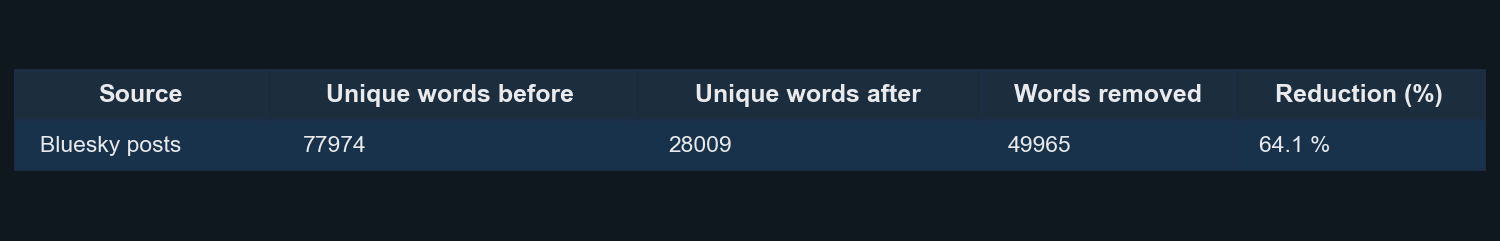
\includegraphics[width=\textwidth]{figures/bluesky/tables/prep_df.png}
\caption{Bluesky preprocessing: vocabulary reduction after cleaning.}
\label{tab:bsky_prep}
\end{table}

\begin{table}[H]
\centering
\small
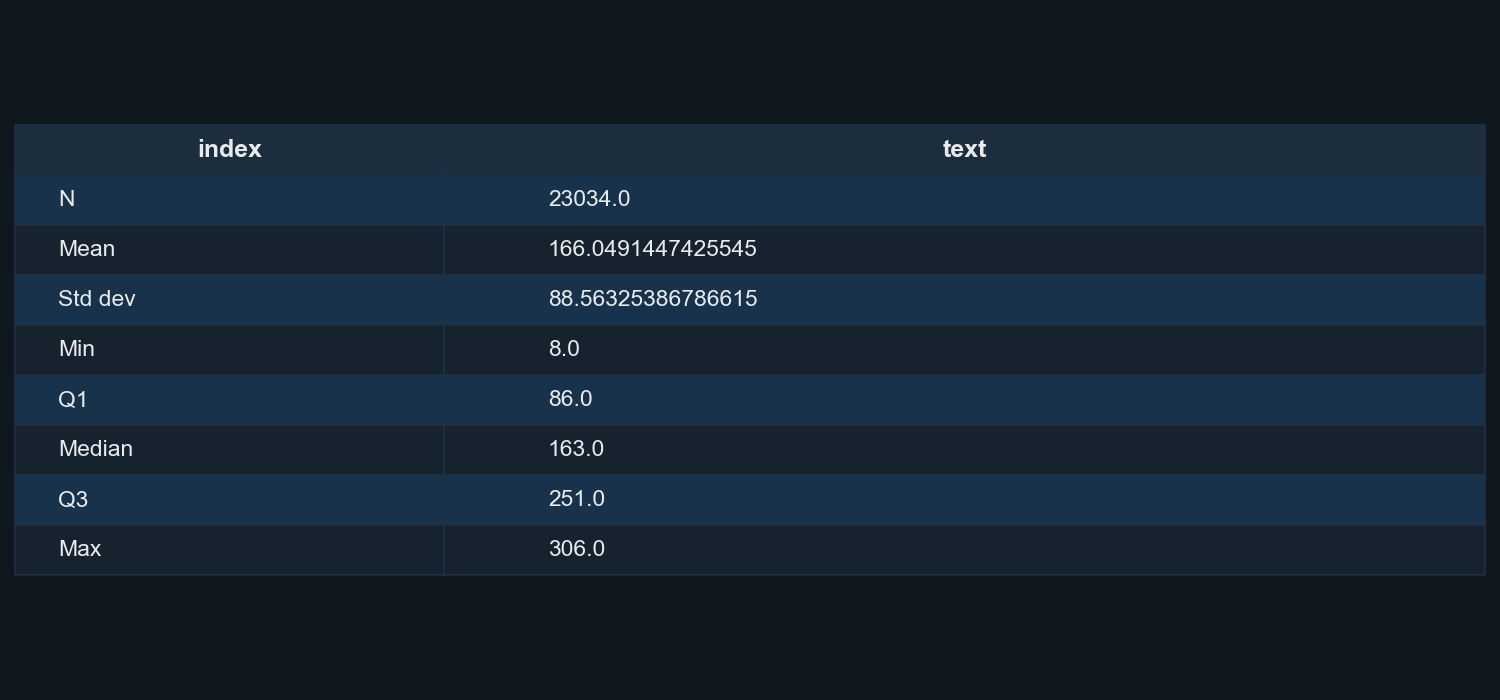
\includegraphics[width=\textwidth]{figures/bluesky/tables/stats.png}
\caption{Bluesky post-length summary after cleaning.}
\label{tab:bsky_stats}
\end{table}

\subsubsection{TF-IDF}

\begin{table}[H]
\centering
\small
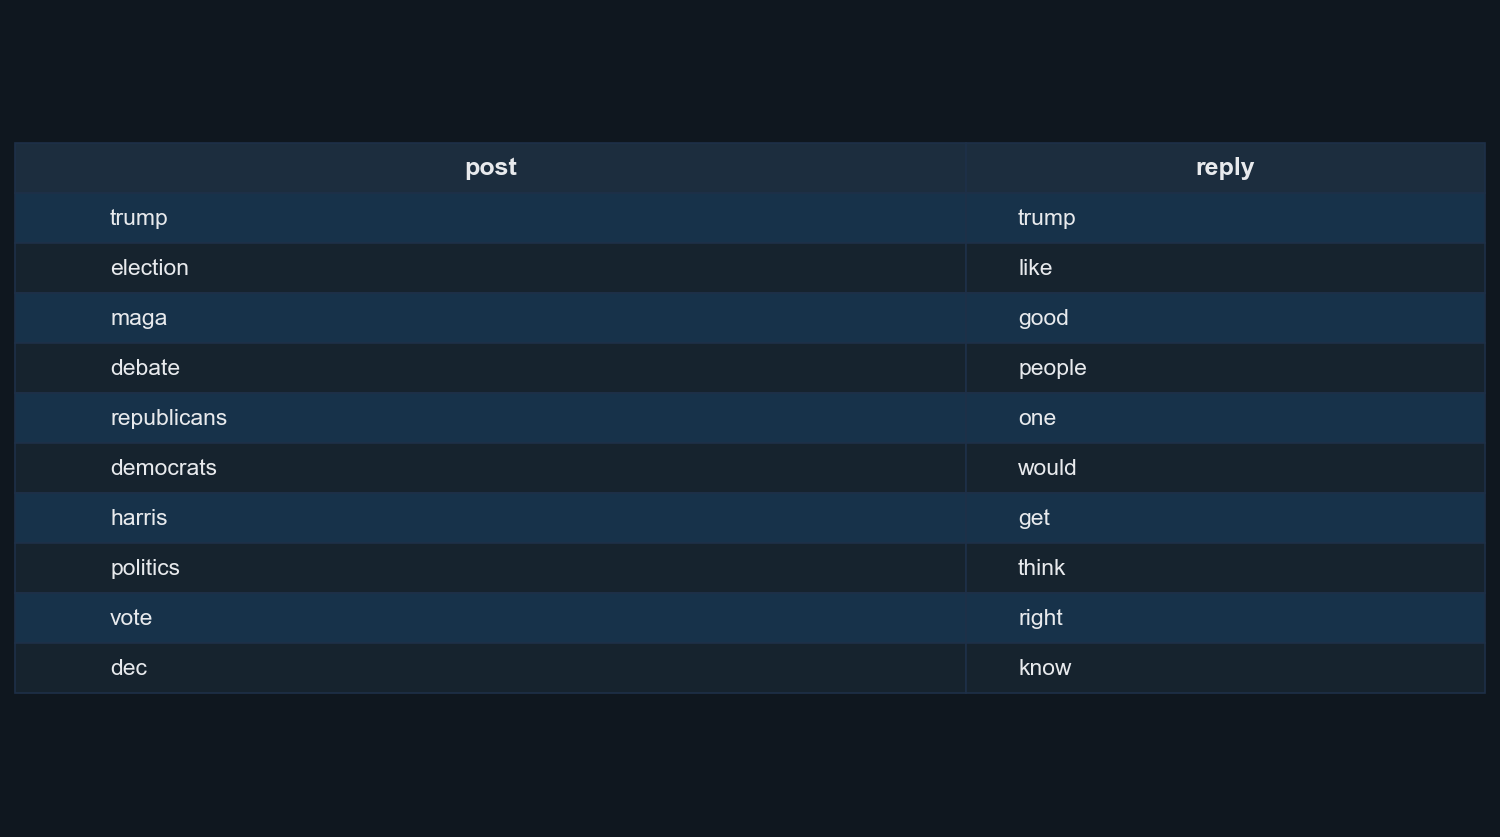
\includegraphics[width=\textwidth]{figures/bluesky/tables/pt_df.png}
\caption{Bluesky post type balance and leading distinctive terms.}
\label{tab:bsky_pt}
\end{table}

\begin{figure}[H]
\centering

\includegraphics[width=\textwidth]{3_tfidf_buzzgroups.png}
\caption{Top 25 distinctive TF-IDF terms per Bluesky buzz group.}
\label{fig:bsky_tfidf_buzzgroups}
\end{figure}

\begin{table}[H]
\centering
\small
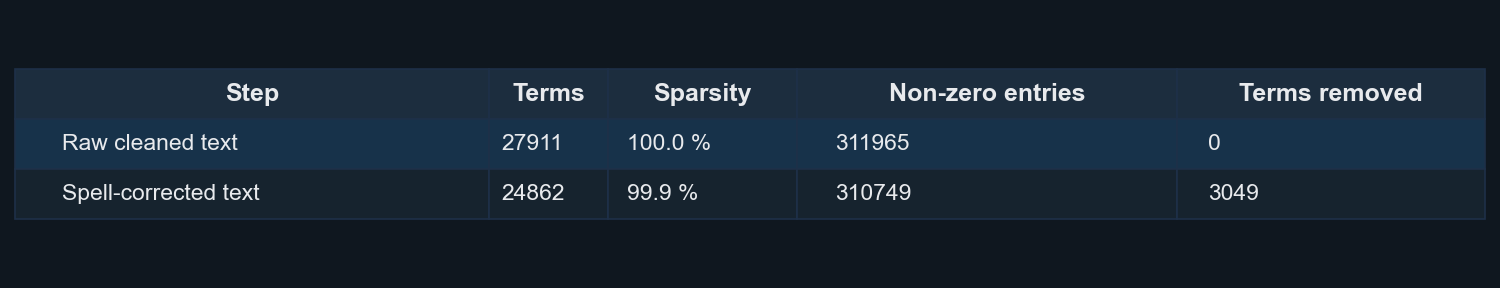
\includegraphics[width=\textwidth]{figures/bluesky/tables/dtm_compare.png}
\caption{Bluesky TF-IDF document-term matrix before and after spell correction.}
\label{tab:bsky_dtm_compare}
\end{table}

\subsubsection{SVD}

\begin{figure}[H]
\centering

\includegraphics[width=\textwidth]{4_svd_variance.png}
\caption{SVD scree plot and cumulative variance for the Bluesky TF-IDF matrix.}
\label{fig:bsky_svd_variance}
\end{figure}

\begin{table}[H]
\centering
\small
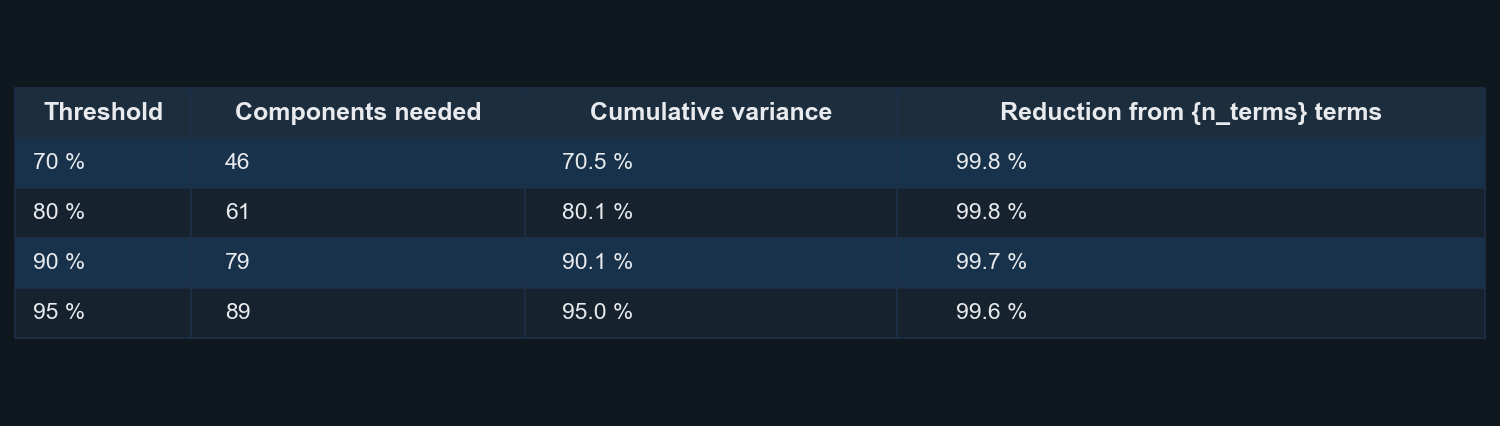
\includegraphics[width=\textwidth]{figures/bluesky/tables/thr_df.png}
\caption{Bluesky SVD thresholds for explained variance.}
\label{tab:bsky_thr}
\end{table}

\begin{table}[H]
\centering
\small
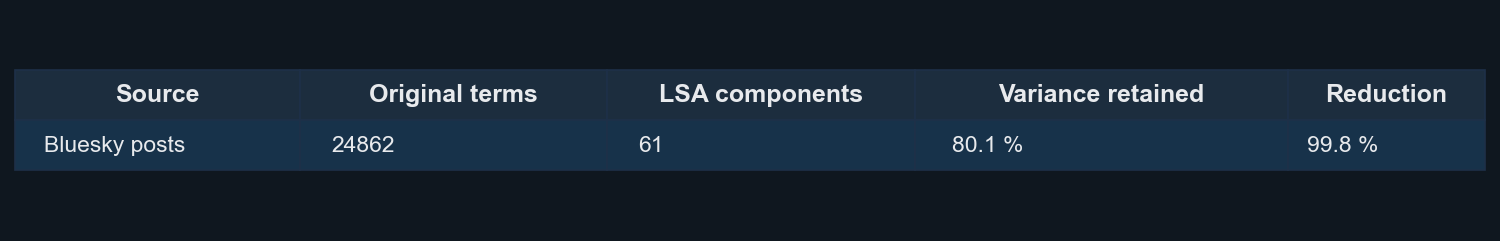
\includegraphics[width=\textwidth]{figures/bluesky/tables/lsa_summary.png}
\caption{Bluesky LSA dimensionality reduction summary.}
\label{tab:bsky_lsa_summary}
\end{table}

\subsubsection{LSA}

\begin{figure}[H]
\centering

\includegraphics[width=\textwidth]{5_lsa_concepts_time.png}
\caption{Latent Semantic Analysis concept trajectories over time.}
\label{fig:bsky_lsa_time}
\end{figure}

\begin{table}[H]
\centering
\small
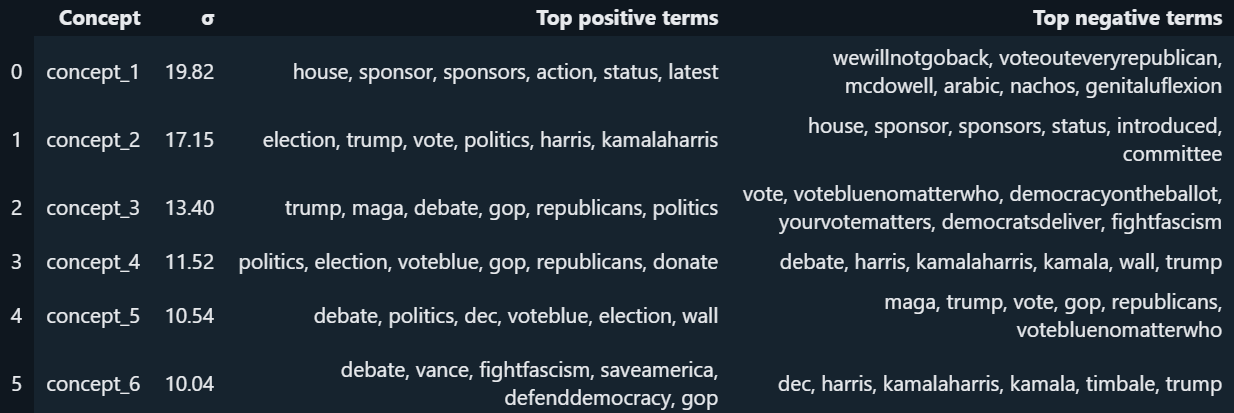
\includegraphics[width=\textwidth]{figures/bluesky/tables/concept_df.png}
\caption{Bluesky LSA concepts and dominant loading terms.}
\label{tab:bsky_concepts}
\end{table}

\subsubsection{Key Terms}

\begin{figure}[H]
\centering

\includegraphics[width=\textwidth,height=0.88\textheight,keepaspectratio]{6_keyterm_frequency.png}
\caption{Weekly frequency of the most salient Bluesky key terms.}
\label{fig:bsky_keyterm_frequency}
\end{figure}

\subsubsection{Word Clouds}

\begin{figure}[H]
\centering

\includegraphics[width=\textwidth]{7_wordclouds.png}
\caption{Bluesky word clouds by buzz group.}
\label{fig:bsky_wordclouds}
\end{figure}

% ==================================================================
\newpage
\subsection{NLP}

% ------------------------------------------------------------------
\subsubsection{Bluesky LDA Setup}

\begin{figure}[H]
\centering

\includegraphics[width=\textwidth]{tables/nlp_preprocessing.png}
\caption{Bluesky LDA preprocessing pipeline summary, documenting tokenization, filtering, and document preparation steps.}
\label{fig:bsky_nlp_preprocessing}
\end{figure}

\begin{table}[H]
\centering
\small

\includegraphics[width=\textwidth]{tables/nlp_dictionary.png}
\caption{Bluesky vocabulary size and filtering metrics for LDA topic modeling.}
\label{tab:bsky_nlp_dictionary}
\end{table}

% ------------------------------------------------------------------
\subsubsection{Bluesky LDA Model Selection}

\begin{figure}[H]
\centering

\includegraphics[width=\textwidth]{tables/nlp_coherence_sweep.png}
\caption{Coherence (u\_mass) and AIC scores across topic range $K=2$ to $10$, with $K=4$ selected as optimal.}
\label{fig:bsky_nlp_coherence_sweep}
\end{figure}

\begin{table}[H]
\centering
\small

\includegraphics[width=\textwidth]{tables/nlp_model_summary.png}
\caption{Final LDA model parameters and training metrics for Bluesky posts.}
\label{tab:bsky_nlp_model_summary}
\end{table}

\begin{table}[H]
\centering
\small

\includegraphics[width=\textwidth]{tables/nlp_topic_words.png}
\caption{Top 10 terms and maximum weight for each of the 4 LDA topics.}
\label{tab:bsky_nlp_topic_words}
\end{table}

% ------------------------------------------------------------------
\subsubsection{Bluesky LDA Outputs}

\begin{figure}[H]
\centering

\includegraphics[width=\textwidth]{nlp_2_wordclouds.png}
\caption{Topic-specific word clouds derived from LDA topic modeling on Bluesky posts, illustrating the semantic content and relative word importance within each of the four identified topics.}
\label{fig:bsky_nlp_wordclouds}
\end{figure}

\begin{figure}[H]
\centering

\includegraphics[width=\textwidth]{nlp_3_topics_time.png}
\caption{Topic prominence over time on Bluesky (7-day rolling mean percentage of daily posts), demonstrating how topic composition evolved across the 2024 US election campaign with marked shifts corresponding to major events.}
\label{fig:bsky_nlp_topics_time}
\end{figure}

\begin{figure}[H]
\centering

\includegraphics[width=\textwidth]{nlp_4_topics_buzzgroup.png}
\caption{Topic distribution across buzz clusters (TrumpBuzz, HarrisBuzz, ElectionBuzz), highlighting how candidate-specific discourse clusters preferentially engage with distinct topic dimensions and revealing homophilic topic preferences.}
\label{fig:bsky_nlp_topics_buzz}
\end{figure}

% ------------------------------------------------------------------
\subsubsection{Newspapers NLP}

\begin{figure}[H]
\centering

\includegraphics[width=\textwidth]{key_mentions_over_time_NER.png}
\caption{Named-entity mention counts over time in newspaper headlines, tracking
key political figures extracted via NER (July--November 2024).}
\label{fig:news_ner_mentions}
\end{figure}

% ==================================================================
\newpage
\subsection{Sentiment Analysis}

% ------------------------------------------------------------------
\subsubsection{VADER}

\begin{figure}[H]
\centering

\includegraphics[width=\textwidth]{vader_bluesky.png}
\caption{VADER compound sentiment scores for Bluesky posts, comparing TrumpBuzz and HarrisBuzz clusters over the campaign period.}
\label{fig:bsky_vader}
\end{figure}

\begin{figure}[H]
\centering

\includegraphics[width=\textwidth]{vader_news.png}
\caption{Daily average VADER sentiment score for newspaper headlines by media-leaning group, July--November 2024. Vertical dashed lines mark key campaign events.}
\label{fig:news_vader}
\end{figure}

% ------------------------------------------------------------------
\subsubsection{TextBlob}

\begin{figure}[H]
\centering

\includegraphics[width=\textwidth]{textblob_bluesky.png}
\caption{TextBlob polarity and subjectivity scores for Bluesky posts by buzz group.}
\label{fig:bsky_textblob}
\end{figure}

\begin{figure}[H]
\centering

\includegraphics[width=\textwidth]{textblob_news.png}
\caption{TextBlob sentiment scores for newspaper headlines by media leaning.}
\label{fig:news_textblob}
\end{figure}

% ------------------------------------------------------------------
\subsubsection{NRCLex}

\begin{figure}[H]
\centering
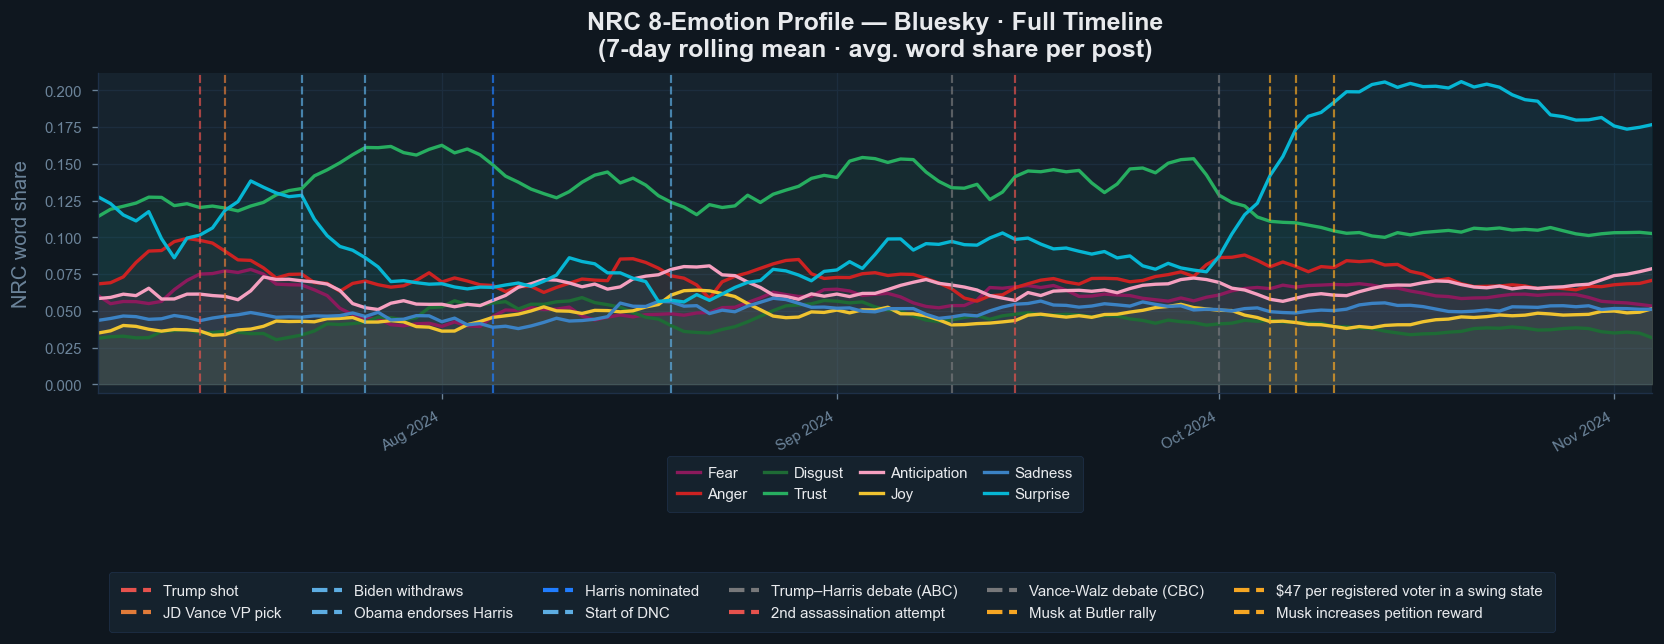
\includegraphics[width=\textwidth]{../figures/bluesky/NRC.png}
\caption{NRC emotion scores for Bluesky posts, showing the eight-emotion breakdown for TrumpBuzz and HarrisBuzz clusters.}
\label{fig:bluesky_nrc}
\end{figure}

\begin{figure}[H]
\centering

\includegraphics[width=\textwidth,height=0.38\textheight,keepaspectratio]{../figures/news/NRC.png}

\vspace{1.2em}


\includegraphics[width=\textwidth,height=0.38\textheight,keepaspectratio]{NRCle_ emotionscores.png}
\caption{Top: NRC emotion scores for newspaper headlines across media leanings.
Bottom: NRCLex eight-emotion profiles by media leaning (Plutchik wheel).}
\label{fig:news_nrc}
\end{figure}

% ------------------------------------------------------------------
\subsubsection{Twitter RoBERTa}

\begin{figure}[H]
\centering

\includegraphics[width=\textwidth]{twitter_roberta_bluesky.png}
\caption{Twitter RoBERTa sentiment scores for Bluesky posts, comparing TrumpBuzz and HarrisBuzz clusters.}
\label{fig:bsky_roberta}
\end{figure}

% ------------------------------------------------------------------
\subsubsection{Combination}

\begin{figure}[H]
\centering

\includegraphics[width=\textwidth]{comparision_sentiment.png}
\caption{Comparison of sentiment methods (VADER, FinBERT, TextBlob) on newspaper headlines.}
\label{fig:news_sentiment_methods}
\end{figure}

% ==================================================================
\newpage
\subsection{Predictive Modeling}

% ---- Table: Hyperparameter Grids ----
\begin{table}[H]
\centering
\caption{Hyperparameter search grids used in walk-forward cross-validation tuning.}
\label{tab:hyperparam_grids}
\small
\begin{tabular}{p{2cm} p{2.5cm} p{4.5cm} p{3cm} p{2.5cm}}
\toprule
\textbf{Model} & \textbf{Hyperparameter} & \textbf{Search Grid} & \textbf{Fixed Parameters} & \textbf{Scaling} \\
\midrule
Ridge & $\alpha$ (L2 penalty) & [0.001, 0.01, 0.1, 1, 10, 100, 500, 1000, 5000, 10000] & --- & Yes (StandardScaler on train fold only) \\[3pt]
Random Forest & \texttt{max\_depth}, \texttt{min\_samples\_leaf} & max\_depth: [2, 3, 4, 5]; min\_samples\_leaf: [1, 2, 3, 5] & n\_estimators=200, random\_state=42 & No (scale-invariant) \\[3pt]
SVM & kernel, $C$, $\varepsilon$ & kernel: [linear, rbf, poly, sigmoid]; $C$: [0.1, 1, 10, 100]; $\varepsilon$: [0.0001, 0.001, 0.01, 0.05] & $\gamma$=scale & Yes (StandardScaler on train fold only) \\[3pt]
\bottomrule
\end{tabular}
\begin{minipage}{\linewidth}
\vspace{2pt}\small\textit{Note: The same search grids are applied across all eight feature sets. Best hyperparameters are selected by minimum mean CV MAE across the 3 walk-forward folds. The test set is completely untouched during tuning.}
\end{minipage}
\end{table}

% ---- Table: Feature Sets ----
\begin{table}[H]
\centering
\caption{Feature sets used in the predictive modelling experiments.}
\label{tab:feature_sets}
\small
\begin{tabular}{c p{2.5cm} c p{3cm} p{5.5cm}}
\toprule
\textbf{\#} & \textbf{Feature Set} & \textbf{\# Features} & \textbf{Sources Included} & \textbf{Description} \\
\midrule
1 & Lag (2f) & 2 & Autoregressive (Polymarket) & Minimal autoregressive baseline: yesterday's Polymarket probability and its 2-day lag. Tests whether the odds series alone contains predictive signal. \\[3pt]
2 & Social (61f) & 61 & Bluesky, Reddit & All Bluesky and Reddit features: daily post volumes, engagement metrics, RoBERTa/VADER sentiment scores, and NRCLex emotion scores per buzz group (Trump, Harris, Election). \\[3pt]
3 & Web+Polls (19f) & 19 & Google Trends, Polls & Google Trends search interest for 10 election-related keywords and 9 polling features (daily averages, rolling averages, margin momentum, polling uncertainty). \\[3pt]
4 & Traditional (19f) & 19 & Newspapers (Media Cloud) & Traditional media features: article counts by political leaning and buzz group, VADER sentiment per leaning, NRCLex emotions, and derived sentiment gap features. \\[3pt]
5 & Financial (10f) & 10 & Financial markets & Five market indicators (S\&P 500, oil, VIX, 10-year bond yield, USD index) and five derived return/volatility features. \\[3pt]
6 & Lag+Social (64f) & 64 & Autoregressive, Bluesky, Reddit & Combination of the autoregressive lag features and all social media features. Tests whether social media adds signal on top of the price series. \\[3pt]
7 & Lag+Soc+Trad (83f) & 83 & Autoregressive, Bluesky, Reddit, Newspapers & Extension of Lag+Social with traditional media features added. Combines social and news signals with the autoregressive baseline. \\[3pt]
8 & Full (111f) & 111 & All sources & All 111 features from the preprocessed basetable (excluding date, target, and lag-1 target). Includes social media, traditional media, Google Trends, polls, financials, and all lag features. \\[3pt]
\bottomrule
\end{tabular}
\end{table}

% ---- Table: Feature Overview ----
\raggedbottom
\begin{longtable}{>{\centering\arraybackslash}p{0.9cm} p{2cm} p{4cm} p{7.5cm}}
\caption{Complete feature overview used in the predictive modelling pipeline.}
\label{tab:feature_overview} \\
\toprule
\textbf{\#} & \textbf{Source} & \textbf{Feature Name} & \textbf{Description} \\
\midrule
\endfirsthead
\toprule
\textbf{\#} & \textbf{Source} & \textbf{Feature Name} & \textbf{Description} \\
\midrule
\endhead
\midrule \multicolumn{4}{r}{\small\textit{Continued on next page}} \\
\endfoot
\bottomrule
\endlastfoot
\underline{1} & Time & \texttt{days\_to\_election} & Calendar days remaining until election day (Nov 5, 2024) \\
2 & Time & \texttt{is\_weekend} & Binary dummy: 1 if Saturday or Sunday, 0 otherwise \\
3 & Time & \texttt{weekday} & Day of week (0=Monday \ldots{} 6=Sunday) \\
4 & Time & \texttt{campaign\_week} & Week number within the campaign period (starting Jul 5) \\
5 & Time & \texttt{days\_since\_last\_event} & Days elapsed since the most recent major political event \\
6 & Bluesky & \texttt{bsky\_total\_posts} & Total number of Bluesky posts per day \\
7 & Bluesky & \texttt{bsky\_unique\_authors} & Number of unique Bluesky authors posting per day \\
8 & Bluesky & \texttt{bsky\_avg\_likes} & Average likes per post per day \\
9 & Bluesky & \texttt{bsky\_avg\_reposts} & Average reposts per post per day \\
10 & Bluesky & \texttt{bsky\_reply\_ratio} & Share of posts that are replies \\
\underline{11} & Bluesky & \texttt{bsky\_trump\_unique\_authors} & Unique authors posting TrumpBuzz content on Bluesky \\
\underline{12} & Bluesky & \texttt{bsky\_harris\_unique\_authors} & Unique authors posting HarrisBuzz content on Bluesky \\
\underline{13} & Bluesky & \texttt{bsky\_trump\_share} & TrumpBuzz posts as a share of total daily Bluesky posts \\
\underline{14} & Bluesky & \texttt{bsky\_harris\_share} & HarrisBuzz posts as a share of total daily Bluesky posts \\
\underline{15} & Bluesky & \texttt{bsky\_posts\_per\_author} & Average number of posts per unique author per day \\
16 & Bluesky & \texttt{bsky\_trump\_sent\_avg} & Mean RoBERTa sentiment score for TrumpBuzz posts \\
17 & Bluesky & \texttt{bsky\_trump\_sent\_std} & Std. dev. of RoBERTa sentiment for TrumpBuzz posts \\
18 & Bluesky & \texttt{bsky\_trump\_pos\_share} & Share of TrumpBuzz posts classified as positive \\
19 & Bluesky & \texttt{bsky\_trump\_neg\_share} & Share of TrumpBuzz posts classified as negative \\
\underline{20} & Bluesky & \texttt{bsky\_trump\_fear} & Mean NRCLex fear score --- Bluesky TrumpBuzz \\
21 & Bluesky & \texttt{bsky\_trump\_anger} & Mean NRCLex anger score --- Bluesky TrumpBuzz \\
22 & Bluesky & \texttt{bsky\_trump\_anticipation} & Mean NRCLex anticipation score --- Bluesky TrumpBuzz \\
\underline{23} & Bluesky & \texttt{bsky\_trump\_trust} & Mean NRCLex trust score --- Bluesky TrumpBuzz \\
\underline{24} & Bluesky & \texttt{bsky\_trump\_surprise} & Mean NRCLex surprise score --- Bluesky TrumpBuzz \\
\underline{25} & Bluesky & \texttt{bsky\_trump\_sadness} & Mean NRCLex sadness score --- Bluesky TrumpBuzz \\
\underline{26} & Bluesky & \texttt{bsky\_trump\_disgust} & Mean NRCLex disgust score --- Bluesky TrumpBuzz \\
\underline{27} & Bluesky & \texttt{bsky\_trump\_joy} & Mean NRCLex joy score --- Bluesky TrumpBuzz \\
\underline{28} & Bluesky & \texttt{bsky\_harris\_sent\_avg} & Mean RoBERTa sentiment score for HarrisBuzz posts \\
29 & Bluesky & \texttt{bsky\_harris\_sent\_std} & Std. dev. of RoBERTa sentiment for HarrisBuzz posts \\
\underline{30} & Bluesky & \texttt{bsky\_harris\_pos\_share} & Share of HarrisBuzz posts classified as positive \\
\underline{31} & Bluesky & \texttt{bsky\_harris\_neg\_share} & Share of HarrisBuzz posts classified as negative \\
\underline{32} & Bluesky & \texttt{bsky\_harris\_fear} & Mean NRCLex fear score --- Bluesky HarrisBuzz \\
\underline{33} & Bluesky & \texttt{bsky\_harris\_anger} & Mean NRCLex anger score --- Bluesky HarrisBuzz \\
\underline{34} & Bluesky & \texttt{bsky\_harris\_anticipation} & Mean NRCLex anticipation score --- Bluesky HarrisBuzz \\
\underline{35} & Bluesky & \texttt{bsky\_harris\_trust} & Mean NRCLex trust score --- Bluesky HarrisBuzz \\
36 & Bluesky & \texttt{bsky\_harris\_surprise} & Mean NRCLex surprise score --- Bluesky HarrisBuzz \\
37 & Bluesky & \texttt{bsky\_harris\_sadness} & Mean NRCLex sadness score --- Bluesky HarrisBuzz \\
\underline{38} & Bluesky & \texttt{bsky\_harris\_disgust} & Mean NRCLex disgust score --- Bluesky HarrisBuzz \\
\underline{39} & Bluesky & \texttt{bsky\_harris\_joy} & Mean NRCLex joy score --- Bluesky HarrisBuzz \\
\underline{40} & Bluesky & \texttt{bsky\_election\_sent\_avg} & Mean RoBERTa sentiment score for ElectionBuzz posts \\
\underline{41} & Bluesky & \texttt{bsky\_election\_sent\_std} & Std. dev. of RoBERTa sentiment for ElectionBuzz posts \\
\underline{42} & Bluesky & \texttt{bsky\_election\_pos\_share} & Share of ElectionBuzz posts classified as positive \\
\underline{43} & Bluesky & \texttt{bsky\_election\_neg\_share} & Share of ElectionBuzz posts classified as negative \\
44 & Bluesky & \texttt{bsky\_election\_fear} & Mean NRCLex fear score --- Bluesky ElectionBuzz \\
45 & Bluesky & \texttt{bsky\_election\_anger} & Mean NRCLex anger score --- Bluesky ElectionBuzz \\
46 & Bluesky & \texttt{bsky\_election\_anticipation} & Mean NRCLex anticipation score --- Bluesky ElectionBuzz \\
47 & Bluesky & \texttt{bsky\_election\_trust} & Mean NRCLex trust score --- Bluesky ElectionBuzz \\
\underline{48} & Bluesky & \texttt{bsky\_election\_surprise} & Mean NRCLex surprise score --- Bluesky ElectionBuzz \\
49 & Bluesky & \texttt{bsky\_election\_sadness} & Mean NRCLex sadness score --- Bluesky ElectionBuzz \\
50 & Bluesky & \texttt{bsky\_election\_disgust} & Mean NRCLex disgust score --- Bluesky ElectionBuzz \\
\underline{51} & Bluesky & \texttt{bsky\_election\_joy} & Mean NRCLex joy score --- Bluesky ElectionBuzz \\
\underline{52} & Bluesky & \texttt{bsky\_sentiment\_gap} & RoBERTa sentiment difference: Trump minus Harris (Bluesky) \\
\underline{53} & Bluesky & \texttt{bsky\_sentiment\_gap\_lag1} & Bluesky sentiment gap (Trump - Harris) lagged 1 day \\
54 & Reddit & \texttt{reddit\_total\_posts} & Total number of Reddit posts per day \\
\underline{55} & Reddit & \texttt{reddit\_unique\_authors} & Number of unique Reddit authors posting per day \\
\underline{56} & Reddit & \texttt{reddit\_avg\_score} & Average post score (upvotes minus downvotes) per day \\
\underline{57} & Reddit & \texttt{reddit\_avg\_upvote\_ratio} & Average upvote ratio per post per day \\
\underline{58} & Reddit & \texttt{reddit\_avg\_comments} & Average number of comments per post per day \\
59 & Reddit & \texttt{reddit\_trump\_unique\_authors} & Unique authors posting TrumpBuzz content on Reddit \\
\underline{60} & Reddit & \texttt{reddit\_harris\_unique\_authors} & Unique authors posting HarrisBuzz content on Reddit \\
61 & Reddit & \texttt{reddit\_trump\_share} & TrumpBuzz posts as a share of total daily Reddit posts \\
\underline{62} & Reddit & \texttt{reddit\_harris\_share} & HarrisBuzz posts as a share of total daily Reddit posts \\
\underline{63} & Reddit & \texttt{reddit\_conservative\_share} & Share of posts from conservative/Trump subreddits \\
64 & Reddit & \texttt{reddit\_liberal\_share} & Share of posts from liberal/Democrat subreddits \\
\underline{65} & Reddit & \texttt{reddit\_posts\_per\_author} & Average posts per unique author per day (Reddit) \\
\underline{66} & Reddit & \texttt{reddit\_trump\_sent\_avg} & Mean VADER compound sentiment for TrumpBuzz posts \\
\underline{67} & Reddit & \texttt{reddit\_trump\_sent\_std} & Std. dev. of VADER sentiment for TrumpBuzz posts \\
\underline{68} & Reddit & \texttt{reddit\_trump\_fear} & Mean NRCLex fear score --- Reddit TrumpBuzz \\
\underline{69} & Reddit & \texttt{reddit\_trump\_anger} & Mean NRCLex anger score --- Reddit TrumpBuzz \\
\underline{70} & Reddit & \texttt{reddit\_trump\_anticipation} & Mean NRCLex anticipation score --- Reddit TrumpBuzz \\
\underline{71} & Reddit & \texttt{reddit\_trump\_trust} & Mean NRCLex trust score --- Reddit TrumpBuzz \\
\underline{72} & Reddit & \texttt{reddit\_trump\_surprise} & Mean NRCLex surprise score --- Reddit TrumpBuzz \\
\underline{73} & Reddit & \texttt{reddit\_trump\_sadness} & Mean NRCLex sadness score --- Reddit TrumpBuzz \\
\underline{74} & Reddit & \texttt{reddit\_trump\_disgust} & Mean NRCLex disgust score --- Reddit TrumpBuzz \\
\underline{75} & Reddit & \texttt{reddit\_trump\_joy} & Mean NRCLex joy score --- Reddit TrumpBuzz \\
76 & Reddit & \texttt{reddit\_harris\_sent\_avg} & Mean VADER compound sentiment for HarrisBuzz posts \\
\underline{77} & Reddit & \texttt{reddit\_harris\_sent\_std} & Std. dev. of VADER sentiment for HarrisBuzz posts \\
78 & Reddit & \texttt{reddit\_harris\_fear} & Mean NRCLex fear score --- Reddit HarrisBuzz \\
79 & Reddit & \texttt{reddit\_harris\_anger} & Mean NRCLex anger score --- Reddit HarrisBuzz \\
\underline{80} & Reddit & \texttt{reddit\_harris\_anticipation} & Mean NRCLex anticipation score --- Reddit HarrisBuzz \\
\underline{81} & Reddit & \texttt{reddit\_harris\_trust} & Mean NRCLex trust score --- Reddit HarrisBuzz \\
82 & Reddit & \texttt{reddit\_harris\_surprise} & Mean NRCLex surprise score --- Reddit HarrisBuzz \\
\underline{83} & Reddit & \texttt{reddit\_harris\_sadness} & Mean NRCLex sadness score --- Reddit HarrisBuzz \\
\underline{84} & Reddit & \texttt{reddit\_harris\_disgust} & Mean NRCLex disgust score --- Reddit HarrisBuzz \\
\underline{85} & Reddit & \texttt{reddit\_harris\_joy} & Mean NRCLex joy score --- Reddit HarrisBuzz \\
86 & Reddit & \texttt{reddit\_election\_sent\_avg} & Mean VADER compound sentiment for ElectionBuzz posts \\
\underline{87} & Reddit & \texttt{reddit\_election\_sent\_std} & Std. dev. of VADER sentiment for ElectionBuzz posts \\
\underline{88} & Reddit & \texttt{reddit\_election\_fear} & Mean NRCLex fear score --- Reddit ElectionBuzz \\
\underline{89} & Reddit & \texttt{reddit\_election\_anger} & Mean NRCLex anger score --- Reddit ElectionBuzz \\
\underline{90} & Reddit & \texttt{reddit\_election\_anticipation} & Mean NRCLex anticipation score --- Reddit ElectionBuzz \\
91 & Reddit & \texttt{reddit\_election\_trust} & Mean NRCLex trust score --- Reddit ElectionBuzz \\
\underline{92} & Reddit & \texttt{reddit\_election\_surprise} & Mean NRCLex surprise score --- Reddit ElectionBuzz \\
\underline{93} & Reddit & \texttt{reddit\_election\_sadness} & Mean NRCLex sadness score --- Reddit ElectionBuzz \\
94 & Reddit & \texttt{reddit\_election\_disgust} & Mean NRCLex disgust score --- Reddit ElectionBuzz \\
\underline{95} & Reddit & \texttt{reddit\_election\_joy} & Mean NRCLex joy score --- Reddit ElectionBuzz \\
\underline{96} & Reddit & \texttt{reddit\_sentiment\_gap} & VADER sentiment difference: Trump minus Harris (Reddit) \\
\underline{97} & Reddit & \texttt{reddit\_sentiment\_gap\_lag1} & Reddit sentiment gap (Trump - Harris) lagged 1 day \\
98 & Newspapers & \texttt{news\_total} & Total number of news articles per day \\
99 & Newspapers & \texttt{news\_trump\_count} & Daily article count classified as TrumpBuzz \\
100 & Newspapers & \texttt{news\_harris\_count} & Daily article count classified as HarrisBuzz \\
\underline{101} & Newspapers & \texttt{news\_election\_count} & Daily article count classified as ElectionBuzz \\
102 & Newspapers & \texttt{news\_rep\_count} & Articles from Republican-leaning outlets \\
103 & Newspapers & \texttt{news\_dem\_count} & Articles from Democratic-leaning outlets \\
104 & Newspapers & \texttt{news\_cen\_count} & Articles from Center/Unknown-leaning outlets \\
105 & Newspapers & \texttt{news\_trump\_share} & Trump articles as a share of total daily articles \\
106 & Newspapers & \texttt{news\_harris\_share} & Harris articles as a share of total daily articles \\
107 & Newspapers & \texttt{news\_attention\_asymmetry} & Relative Trump vs. Harris media attention: (Trump - Harris) / total \\
\underline{108} & Newspapers & \texttt{news\_attention\_asymmetry\_7d} & 7-day rolling average of the attention asymmetry \\
109 & Newspapers & \texttt{news\_attention\_asymmetry\_lag1} & News attention asymmetry lagged 1 day \\
110 & Newspapers & \texttt{news\_attention\_asymmetry\_7d\_lag1} & 7-day rolling news attention asymmetry lagged 1 day \\
\underline{111} & Newspapers & \texttt{vader\_compound\_mean\_dem} & Mean VADER compound sentiment --- Democratic-leaning outlets \\
112 & Newspapers & \texttt{vader\_compound\_mean\_rep} & Mean VADER compound sentiment --- Republican-leaning outlets \\
113 & Newspapers & \texttt{vader\_compound\_mean\_cen} & Mean VADER compound sentiment --- Center/Unknown outlets \\
\underline{114} & Newspapers & \texttt{vader\_compound\_std\_dem} & Std. dev. of VADER sentiment --- Democratic-leaning outlets \\
115 & Newspapers & \texttt{vader\_compound\_std\_rep} & Std. dev. of VADER sentiment --- Republican-leaning outlets \\
116 & Newspapers & \texttt{vader\_compound\_std\_cen} & Std. dev. of VADER sentiment --- Center/Unknown outlets \\
117 & Newspapers & \texttt{vader\_pos\_share\_dem} & Share of positive articles --- Democratic-leaning outlets \\
118 & Newspapers & \texttt{vader\_pos\_share\_rep} & Share of positive articles --- Republican-leaning outlets \\
119 & Newspapers & \texttt{vader\_pos\_share\_cen} & Share of positive articles --- Center/Unknown outlets \\
\underline{120} & Newspapers & \texttt{vader\_neg\_share\_dem} & Share of negative articles --- Democratic-leaning outlets \\
121 & Newspapers & \texttt{vader\_neg\_share\_rep} & Share of negative articles --- Republican-leaning outlets \\
122 & Newspapers & \texttt{vader\_neg\_share\_cen} & Share of negative articles --- Center/Unknown outlets \\
123 & Newspapers & \texttt{nrc\_fear\_dem} & Mean NRCLex fear score --- Democratic-leaning outlets \\
124 & Newspapers & \texttt{nrc\_fear\_rep} & Mean NRCLex fear score --- Republican-leaning outlets \\
\underline{125} & Newspapers & \texttt{nrc\_fear\_cen} & Mean NRCLex fear score --- Center/Unknown outlets \\
126 & Newspapers & \texttt{nrc\_anger\_dem} & Mean NRCLex anger score --- Democratic-leaning outlets \\
127 & Newspapers & \texttt{nrc\_anger\_rep} & Mean NRCLex anger score --- Republican-leaning outlets \\
\underline{128} & Newspapers & \texttt{nrc\_anger\_cen} & Mean NRCLex anger score --- Center/Unknown outlets \\
\underline{129} & Newspapers & \texttt{nrc\_anticipation\_dem} & Mean NRCLex anticipation score --- Democratic-leaning outlets \\
\underline{130} & Newspapers & \texttt{nrc\_anticipation\_rep} & Mean NRCLex anticipation score --- Republican-leaning outlets \\
\underline{131} & Newspapers & \texttt{nrc\_anticipation\_cen} & Mean NRCLex anticipation score --- Center/Unknown outlets \\
132 & Newspapers & \texttt{nrc\_trust\_dem} & Mean NRCLex trust score --- Democratic-leaning outlets \\
133 & Newspapers & \texttt{nrc\_trust\_rep} & Mean NRCLex trust score --- Republican-leaning outlets \\
134 & Newspapers & \texttt{nrc\_trust\_cen} & Mean NRCLex trust score --- Center/Unknown outlets \\
\underline{135} & Newspapers & \texttt{nrc\_surprise\_dem} & Mean NRCLex surprise score --- Democratic-leaning outlets \\
136 & Newspapers & \texttt{nrc\_surprise\_rep} & Mean NRCLex surprise score --- Republican-leaning outlets \\
\underline{137} & Newspapers & \texttt{nrc\_surprise\_cen} & Mean NRCLex surprise score --- Center/Unknown outlets \\
\underline{138} & Newspapers & \texttt{nrc\_sadness\_dem} & Mean NRCLex sadness score --- Democratic-leaning outlets \\
\underline{139} & Newspapers & \texttt{nrc\_sadness\_rep} & Mean NRCLex sadness score --- Republican-leaning outlets \\
\underline{140} & Newspapers & \texttt{nrc\_sadness\_cen} & Mean NRCLex sadness score --- Center/Unknown outlets \\
\underline{141} & Newspapers & \texttt{nrc\_disgust\_dem} & Mean NRCLex disgust score --- Democratic-leaning outlets \\
142 & Newspapers & \texttt{nrc\_disgust\_rep} & Mean NRCLex disgust score --- Republican-leaning outlets \\
143 & Newspapers & \texttt{nrc\_disgust\_cen} & Mean NRCLex disgust score --- Center/Unknown outlets \\
\underline{144} & Newspapers & \texttt{nrc\_joy\_dem} & Mean NRCLex joy score --- Democratic-leaning outlets \\
145 & Newspapers & \texttt{nrc\_joy\_rep} & Mean NRCLex joy score --- Republican-leaning outlets \\
\underline{146} & Newspapers & \texttt{nrc\_joy\_cen} & Mean NRCLex joy score --- Center/Unknown outlets \\
\underline{147} & Newspapers & \texttt{news\_vader\_leaning\_gap} & VADER sentiment gap: Republican-leaning minus Democratic-leaning outlets \\
148 & Newspapers & \texttt{news\_vader\_leaning\_gap\_lag1} & News VADER leaning gap lagged 1 day \\
149 & Newspapers & \texttt{nrc\_fear\_avg} & Average NRCLex fear score across all outlet leanings \\
150 & Newspapers & \texttt{nrc\_anger\_avg} & Average NRCLex anger score across all outlet leanings \\
151 & Newspapers & \texttt{nrc\_trust\_avg} & Average NRCLex trust score across all outlet leanings \\
152 & Newspapers & \texttt{nrc\_anticipation\_avg} & Average NRCLex anticipation score across all outlet leanings \\
\underline{153} & Google Trends & \texttt{gt\_trump} & Daily Google search interest index for 'Trump' \\
\underline{154} & Google Trends & \texttt{gt\_kamala} & Daily Google search interest index for 'Kamala' \\
155 & Google Trends & \texttt{gt\_vance} & Daily Google search interest index for 'Vance' \\
\underline{156} & Google Trends & \texttt{gt\_walz} & Daily Google search interest index for 'Walz' \\
\underline{157} & Google Trends & \texttt{gt\_election\_2024} & Daily Google search interest index for 'election 2024' \\
\underline{158} & Google Trends & \texttt{gt\_trump\_minus\_kamala} & Search gap: Trump index minus Kamala index \\
\underline{159} & Google Trends & \texttt{gt\_trump\_share} & Trump's share of combined Trump + Kamala search interest \\
\underline{160} & Google Trends & \texttt{gt\_trump\_7d} & 7-day rolling average of Trump search interest \\
\underline{161} & Google Trends & \texttt{gt\_kamala\_7d} & 7-day rolling average of Kamala search interest \\
\underline{162} & Google Trends & \texttt{gt\_trump\_lag1} & Google Trends Trump search interest lagged 1 day \\
163 & Google Trends & \texttt{gt\_kamala\_lag1} & Google Trends Kamala search interest lagged 1 day \\
\underline{164} & Google Trends & \texttt{gt\_trump\_share\_lag1} & Google Trends Trump search share lagged 1 day \\
\underline{165} & Polls & \texttt{poll\_trump\_avg} & Daily average Trump poll percentage (forward-filled on days without polls) \\
\underline{166} & Polls & \texttt{poll\_harris\_avg} & Daily average Harris poll percentage (forward-filled on days without polls) \\
\underline{167} & Polls & \texttt{poll\_margin} & Daily average poll margin (Trump minus Harris) \\
168 & Polls & \texttt{poll\_n\_today} & Number of new polls published on that day \\
\underline{169} & Polls & \texttt{poll\_trump\_7d\_avg} & 7-day rolling average of Trump poll share \\
\underline{170} & Polls & \texttt{poll\_harris\_7d\_avg} & 7-day rolling average of Harris poll share \\
\underline{171} & Polls & \texttt{poll\_margin\_7d\_avg} & 7-day rolling average of poll margin \\
172 & Polls & \texttt{poll\_margin\_change\_7d} & 7-day momentum: change in poll margin over the past week \\
\underline{173} & Polls & \texttt{poll\_volatility\_7d} & 7-day rolling std. dev. of poll margin (polling uncertainty) \\
174 & Polls & \texttt{poll\_market\_divergence} & Difference between poll margin and Polymarket implied probability \\
\underline{175} & Polls & \texttt{poll\_margin\_lag1} & Poll margin lagged 1 day \\
\underline{176} & Polls & \texttt{poll\_market\_divergence\_lag1} & Poll-market divergence lagged 1 day \\
177 & Financials & \texttt{sp500} & S\&P 500 closing price \\
\underline{178} & Financials & \texttt{oil} & Crude oil price (USD per barrel) \\
\underline{179} & Financials & \texttt{vix} & CBOE Volatility Index (market fear gauge) \\
\underline{180} & Financials & \texttt{bond\_10y} & US 10-year Treasury bond yield \\
\underline{181} & Financials & \texttt{usd\_index} & US Dollar Index \\
182 & Financials & \texttt{sp500\_return\_1d} & S\&P 500 one-day percentage return \\
\underline{183} & Financials & \texttt{sp500\_return\_7d} & S\&P 500 seven-day percentage return \\
\underline{184} & Financials & \texttt{sp500\_vol\_7d} & 7-day rolling volatility of S\&P 500 daily returns \\
\underline{185} & Financials & \texttt{oil\_return\_1d} & Oil one-day percentage return \\
\underline{186} & Financials & \texttt{vix\_change\_1d} & One-day absolute change in VIX \\
\underline{187} & Financials & \texttt{vix\_lag1} & VIX lagged 1 day \\
188 & Financials & \texttt{sp500\_return\_1d\_lag1} & S\&P 500 one-day return lagged 1 day \\
\underline{189} & Polymarket & \texttt{polymarket\_trump\_prob\_lag1} & Polymarket Trump win probability lagged 1 day \\
190 & Polymarket & \texttt{polymarket\_trump\_prob\_lag2} & Polymarket Trump win probability lagged 2 days \\
191 & Polymarket & \texttt{polymarket\_trump\_prob\_lag3} & Polymarket Trump win probability lagged 3 days \\
\underline{192} & Polymarket & \texttt{polymarket\_trump\_prob\_lag4} & Polymarket Trump win probability lagged 4 days \\
193 & Polymarket & \texttt{polymarket\_trump\_prob\_lag5} & Polymarket Trump win probability lagged 5 days \\
\underline{194} & Polymarket & \texttt{price\_change\_lag1} & Daily price change in Polymarket odds, lagged 1 day \\
195 & Polymarket & \texttt{price\_change\_lag2} & Daily price change in Polymarket odds, lagged 2 days \\
196 & Polymarket & \texttt{price\_change\_lag3} & Daily price change in Polymarket odds, lagged 3 days \\
\end{longtable}
\flushbottom

\begin{figure}[H]
\centering

\includegraphics[width=\textwidth]{predictive/walk_forward_cv.png}
\caption{Walk-forward cross-validation scheme with expanding training windows, preventing look-ahead bias in the time-series prediction task.}
\label{fig:pred_walk_forward_cv}
\end{figure}

\begin{figure}[H]
\centering

\includegraphics[width=\textwidth]{predictive/SVM_result.png}
\caption{Best-performing SVM model predictions on test set (October 22 -- November 4, 2024), showing predicted vs.\ actual Polymarket Trump win probability.}
\label{fig:pred_svm_result}
\end{figure}

\begin{figure}[H]
\centering

\includegraphics[width=\textwidth]{predictive/svm_shap_kernel_explainer.png}
\caption{SHAP kernel explainer analysis for the SVM model, illustrating feature contributions to individual predictions and aggregated feature importance.}
\label{fig:pred_svm_shap}
\end{figure}

\begin{figure}[H]
\centering

\includegraphics[width=\textwidth]{predictive/beeswarm.png}
\caption{Feature importance beeswarm plot showing the distribution of SHAP values across all predictions, with color indicating feature value and position indicating impact on model output.}
\label{fig:pred_beeswarm}
\end{figure}
